\documentclass[border=5pt]{standalone}
\usepackage{tikz}
\usepackage{amsmath}
\usetikzlibrary{calc,intersections}
\usepackage{pgfplots}
\pgfplotsset{compat=1.16}
\usepgfplotslibrary{polar}
\begin{document}
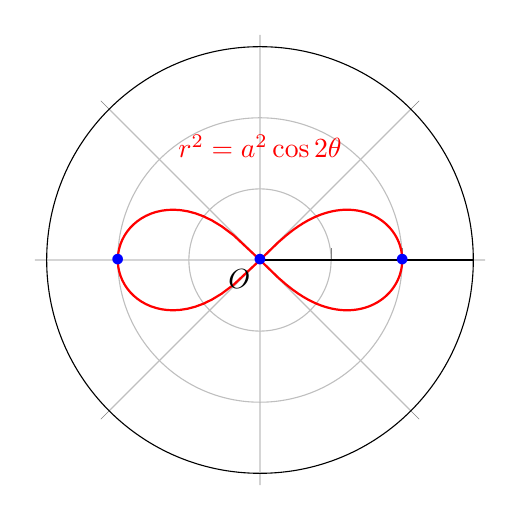
\begin{tikzpicture}
\begin{polaraxis}[
    width=7cm,
    height=7cm,
    grid=both,
    xmin=0, xmax=360,
    ymin=0, ymax=1.5,
    xtick={0,45,...,315},
    ytick={0.5,1},
    xticklabels={},
    yticklabels={},
]
    % Lemniscate
    \addplot[red, thick, domain=0:45, samples=50] {sqrt(cos(2*x))};
    \addplot[red, thick, domain=315:360, samples=50] {sqrt(cos(2*x))};
    \addplot[red, thick, domain=135:225, samples=50] {sqrt(cos(2*x))};

    % Origin
    \node[blue] at (axis cs:0,0) {$\bullet$};
    \node[below left] at (axis cs:0,0) {$O$};

    % Loop endpoints
    \node[blue] at (axis cs:0,1) {$\bullet$};
    \node[blue] at (axis cs:180,1) {$\bullet$};

    % Labels
    \node[red] at (axis cs:90,0.8) {$r^2 = a^2\cos 2\theta$};
\end{polaraxis}
\end{tikzpicture}
\end{document}
